\chapter{Bobine mobile et membrane}
\section{Introduction}
La bobine mobile est reliée à l'output du circuit imprimé et permet de faire bouger la membrane. Elle se situe dans 
l'entrefer. Suivant la direction du courant dans la bobine, direction déteminée par la différence de potentiel
entre les output de la breadboard, la force exercée par le champ magnétique sur celle-ci poussera la 
membrane dans un sens ou dans l'autre.

\section{Hypothèses}
Nous utiliserons les valeurs théoriques obtenues durant la partie précédante sur l'électro-aimant dans nos calculs.
Ainsi, le champ dans l'entrefer $B = 0.1\tesla$, la hauteur de l'entrefer est $h = 0.01\meter$, sa longueur 
$e = 0.005\,\meter$. Nous supposons également que $B$ est uniforme dans l'entrefer. Enfin, nous avons 
calculé que la longueur de fil perpendiculaire au champ par tour de bobine est de $2h$, $h$ étant 
la hauteur de l'entrefer ($h = 0.01\meter$) 

\section{Dévelopement théorique}

\begin{figure}	
\begin{center}
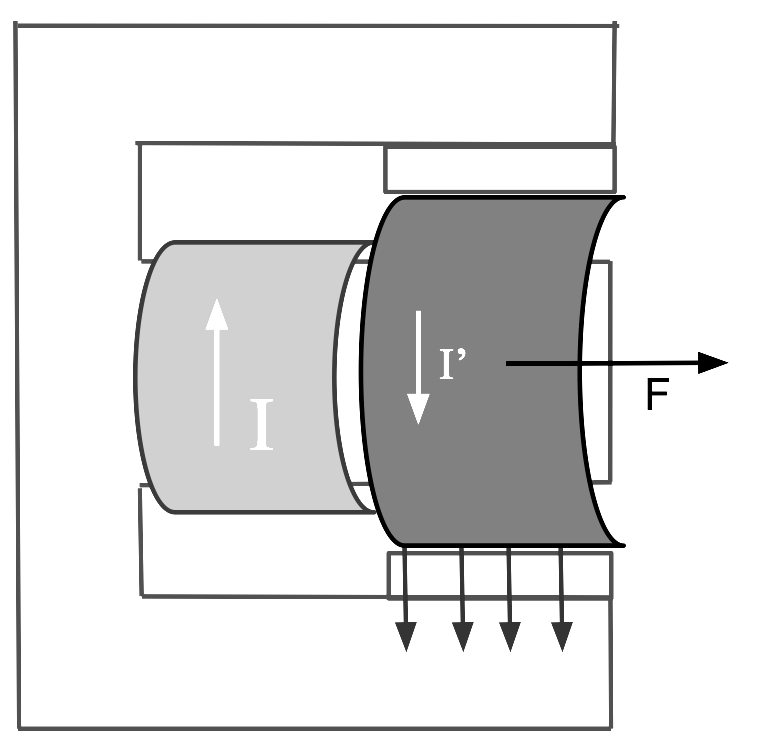
\includegraphics[scale=0.7]{img/bobine-mobile}
\end{center}
\caption{Schema de la bobine mobile}		
\label{fig:bobinemobile}		
\end{figure}

La force exercée par un champ magnétique sur un fil parcouru par un courant est $F =  I' l x B$\, (Force de Laplace). Puisque 
chaque boucle intercepte $2h$ de longueur de fil perpendiculaire, et que la bobine mobile est faite de $N'$, nous pouvons
donc en déduire que $F_{tot} = 2h N' I' * B$ \. Nous avons $B = \frac{\mu_0 N I}{e}$ qui fut déterminé 
lors du chapitre précédent. La force exercée par le champ magnétique sur la bobine est donc 
$ |F_{tot}| = 2 \mu_0 N N' I I' \frac{h}{e}$. La direction de la force dépends du sens du courant dans la bobine, et 
celui ci est déterminé par la différence de potentiel entre les deux output de la plaquette. Selon le courant et son
intensité, la bobine (et donc la membrane liée à celle-ci) sera accélérée dans une direction ou son opposé, reproduisant 
ainsi la bande sonore de la musique.
\section{Calcul}
Si la différence de tension entre les 2 output est de $5\volt$, le courant dans la bobine mobile est de 
$I' = \frac{5\volt}{8\ohm} = 0.625\ampere$ ($8\ohm$ est la résistance totale de la bobine mobile avec une petite 
résistance ajoutée). La force exercée sur la bobine est donc de $F = 0.04 \newton$
\section{Résultats pratiques}
Cette force relativement faible fut suffisante pour obtenir une qualité audio acceptable et un volume correct. 
En minimisant la masse de la bobine mobile (seulement 5\meter de fil utilisé contre 50 pour l'électro-aimant, 
donnant une masse d'environ 16\gram), nous obtenions une grande accélération de $2.5\meter\per\second^2$. 
